\documentclass[11pt]{article}
\usepackage[margin=24mm]{geometry}
\usepackage{graphicx,booktabs,amsmath,siunitx}
\begin{document}
\section*{Averaging scan for the calibrated NAUSICAA readout}
The selected 180 nm circuit has M3 dimensions $200\times2\,\mu\mathrm{m}$,
M4 dimensions $2.88\times1.44\,\mu\mathrm{m}$, external input capacitance
1.25 pF, feedback capacitance 3 fF, supply 1.8 V and temperature 293.15 K.
The transistor models include intrinsic capacitances and thermal and flicker noise.
Uniform ion collection lasts 20 ms; the calibrated discharge time is
2.454158 s. Voltage averages are centred at the frame boundaries.

The input is the finite-gap current of a central trajectory to a 0.5 mm
square pad in an infinite grounded plane, with a homogeneous gas half-space.
The weighting potential is one on the pad, zero on the surrounding plane,
and zero at infinity. The ion moves at 3 m/s over the 5 mm gap. The source
preserves $e[1-\phi_w(g)]$ per ion.

Julia recalculates the signal gain for every averaging width and integrates
the stationary output noise from 0.1 Hz to 1 MHz with the same averaging and
frame-difference filter. The circuit and raw transients are unchanged.
\begin{center}
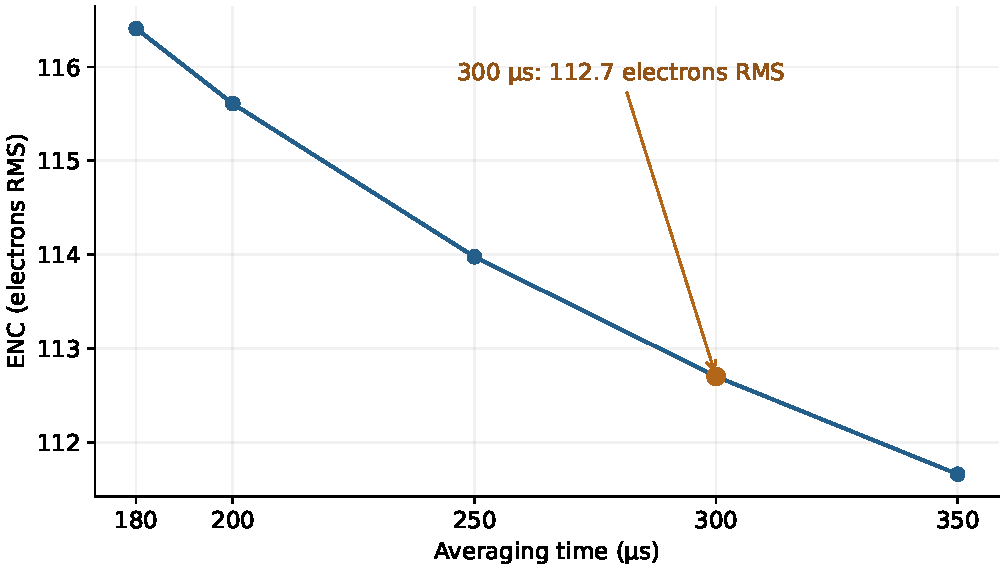
\includegraphics[width=.9\linewidth]{spice_averaging.pdf}
\begin{tabular}{rrrr}\toprule
Average ($\mu$s) & Gain ($\mu$V/ion) & Noise (mV RMS) & ENC ($e$ RMS)\\\midrule
180 & 27.145 & 3.16 & 116.41 \\
200 & 27.141 & 3.138 & 115.61 \\
250 & 27.131 & 3.092 & 113.98 \\
300 & 27.119 & 3.056 & 112.7 \\
350 & 27.107 & 3.027 & 111.66 \\
\bottomrule\end{tabular}\end{center}
The selected 300 $\mu$s point reproduces the saved discharge-calibration gain
and noise to a relative tolerance of $10^{-10}$. Checks halve the transient
step, compare 200 and 400 spectral points per decade and increase quadrature
order from 8 to 16. Maximum relative changes are \num{5.62e-06}, \num{7.97e-07} and \num{5.88e-14},
respectively.

Reproduction: run \texttt{scripts/electronics/readout/build\_averaging\_scan.jl}, then
\texttt{scripts/electronics/readout/plot\_averaging\_scan.py}. The Julia result is
\texttt{results/ltspice/discharge\_calibration/20ms/paper\_readout.h5}.
It records hashes of the raw data, calibration, configuration, analysis and filter.
\end{document}
